\chapter{ランサムウェア}
% 本章では,本研究の提案手法に関連する要素に注目して,ランサムウェアについて説明する.





\section{概要}
\label{sec:ransom-overview}
ランサムウェアとはマルウェアの一種であり,攻撃者が要求した金額が支払われるまで,システムやデータへのアクセスを制限する.
言い換えると,データや計算資源,サービスなどのリソースを人質に取って被害者を脅迫することで身代金を要求するマルウェアがランサムウェアである.

ランサムウェアはリソースへのアクセスを制限する方法に基づいて暗号化ランサムウェアとロッカーランサムウェアに分類される \cite{oz2022survey}.
暗号化ランサムウェアは感染先ホストのファイルやデータを暗号化し,元のファイルを削除または上書きする.
ロッカーランサムウェアは暗号化を行わず,デスクトップのスクリーンやブラウザをロックすることで被害者がシステムを利用できないようにする.
本研究は暗号化ランサムウェアを対象としているため,本稿では暗号化ランサムウェアを単に「ランサムウェア」と呼ぶことにする.

AIDS Trojan \cite{aids-trojan} は1989年に最初のランサムウェアとして登場した.
AIDS Trojanは被害者に郵送されたフロッピーディスクを介して感染し,Windowsシステムを対象としていた.
その後インターネットの普及に伴い,ランサムウェアによる被害が増加し始めた.
2005年に登場したGPCode \cite{PGPCoder42:online} はフィッシングメールを介して感染し,独自の暗号化アルゴリズムによってファイルを暗号化した.

現代のランサムウェアはますます高度化している.
ランサムウェアの進化における重要な要素を以下に列挙する.
\begin{itemize}
  \item AESなどの対称鍵暗号化アルゴリズムやRSA,楕円曲線暗号などの非対称鍵暗号化アルゴリズムを使用して暗号化を行うようになっている \cite{Evolution-Ransomware}.
        これにより,復号鍵を入手することができなければデータの復号はほぼ不可能となった.

  \item Windowsだけでなく,Linux,macOS,Androidなどの他のOSを対象としたランサムウェアも登場するようになった.

  \item ビットコインに代表される仮想通貨が普及したことで身代金の支払いが匿名で行えるようになり,攻撃者の特定が難しくなった.

  \item ランサムウェアの開発と配布を有料で行うサービスであるRansomware as a Service (RaaS) が登場し,専門知識が無くとも容易に攻撃を実施することができるようになった.

  \item 無差別的な攻撃から,特定の高価値な組織 (政府機関や大企業など) を対象とした高度な攻撃に移行しつつある \cite{early-detection}.

\end{itemize}

\section{ランサムウェアの分類}
\subsection{悪意ある振る舞いに基づく分類}
\ref{sec:ransom-overview}節で述べたように,ランサムウェアは被害者が身代金を支払うまでリソースへのアクセスを制限するが,
アクセスを制限する方法には多様性が見られる.
本稿ではOzらの分類 \cite{Evolution-Ransomware} を参照し,その方法として\textbf{暗号化},\textbf{データ破壊},\textbf{データ窃取}を扱う.

暗号化:
ランサムウェアは暗号化鍵を用いてデータを暗号化し,元のデータを削除するか,暗号化後のデータで上書きする.
この時使用する鍵はランサムウェアの実行ファイルに埋め込まれているか,感染先ホスト上で生成されるか,C2サーバとの通信から取得されるかのいずれかである.
ファイルを暗号化するランサムウェアの中には,暗号化の対象とするファイルを限定するものも存在する.
例えばCTB-Locker \cite{ctb-locker} は,被害者にとってより高価値なファイルのみを暗号化するために,
.pdfや.zipなどの拡張子を持つファイルを暗号化対象としている.
また,Jigsaw \cite{byrne2017jigsaw} は10MB以下のファイルのみを暗号化する.
このように,ランサムウェアの一部は暗号化の対象とするファイルを限定することで,
ランサムウェアの活動が検出されるリスクを緩和している \cite{huang2017flashguard}と考えられる.

データ破壊:
破壊活動を目的としているがランサムウェアに擬態して攻撃者の意図を隠蔽しようとするマルウェアが確認されている.
例えば,2017年に発見されたNotPetya \cite{Petya-No22:online} は,ハードディスク全体を暗号化した後,
ビットコインの送金先として無効なアドレスを提示していた.
このアドレスはランダムに生成されており,攻撃者が金銭を回収する意図がないことから,
NotPetyaは破壊活動を目的として作成されたと考えられる \cite{Petya-No22:online}.
同様の攻撃として,暗号化を行わず,ランダムなデータでファイルを上書きするマルウェアを作成し使用することも可能である.
なお,このタイプのマルウェアの被害者は身代金を支払ってもリソースを復旧することができないが,
本研究ではランサムウェアとして扱う.

データ窃取:
ランサムウェアは機密文書や顧客の個人情報などの重要データを摂取する可能性がある.
データの暗号化または破壊とデータの窃取を組み合わせて脅迫を行うランサムウェアを「二重脅迫ランサムウェア」と呼ぶ.
二重脅迫ランサムウェアは,データの復旧のために一回,窃取したデータの公開を防ぐためにもう一回,被害者に身代金を要求する.
二重脅迫ランサムウェアによる被害は近年増加しており,SOPHOS社が発表したレポート \cite{sophos-report:online} によると,
2023年に発生したランサムウェアインシデントのうち32\%においてデータの摂取も発生している.
加えて,データの窃取のみによって脅迫を行う「ノーウェアランサム」\cite{nowhere-ransom} と呼ばれる手法も確認されている.

\section{暗号化アルゴリズムに基づく分類}
データを暗号化するランサムウェアは\textbf{対称鍵暗号化},\textbf{非対称鍵暗号化},\textbf{ハイブリッド暗号化}のいずれかの暗号化技術を採用することができる.
採用する暗号化アルゴリズムは,ISO/IEC \cite{ISOIEC2784:online} などの標準化団体が採択した標準的なアルゴリズムが
使用される場合と,攻撃者によって独自に設計される場合がある.
Begovicら \cite{begovic2023cryptographic} が調査した,1991年から2021年までに確認された著名なランサムウェア変種の
暗号化アルゴリズムの使用状況を\figref{fig:encrypt_algo}に示す.

\begin{figure}[tb]
  \begin{center}
    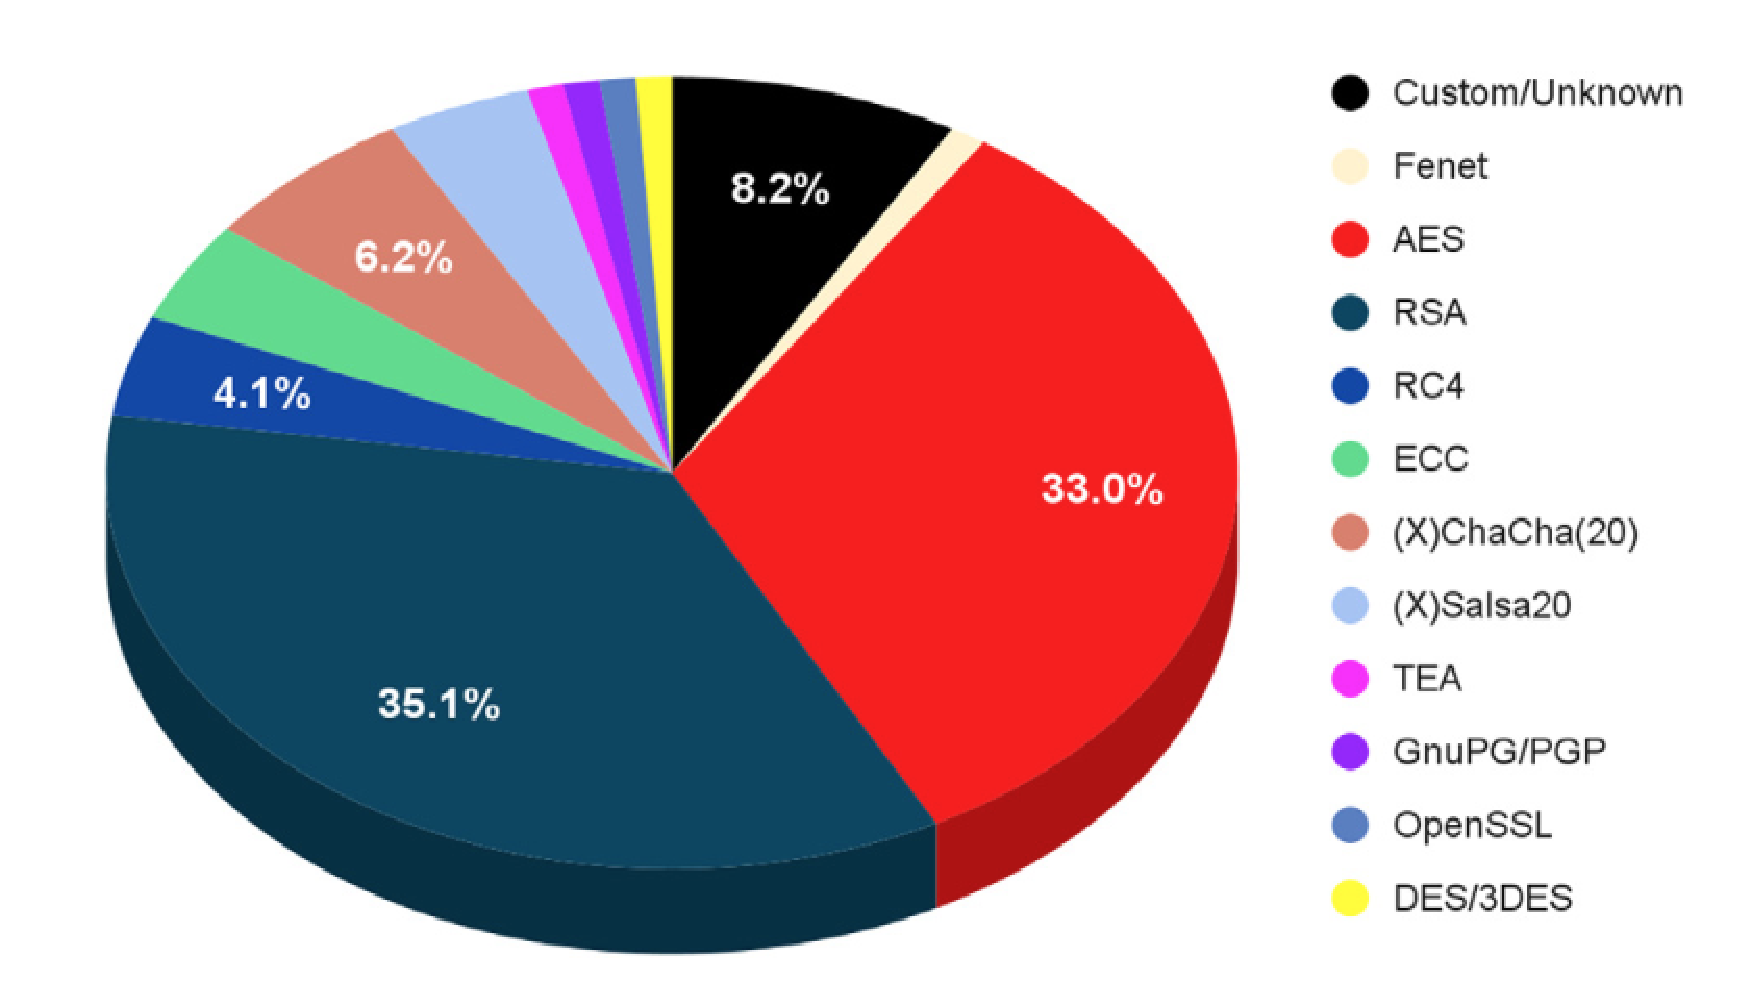
\includegraphics[width=0.8\columnwidth]{./doc/img/encrypt_algo.eps}
  \end{center}
  \caption{foobar}
  \label{fig:encrypt_algo}
\end{figure}




